\chapter{The Peccei--Quinn Axion Solution}


The most famous resolution to the strong \CP\ problem is the Peccei--Quinn theory of the \emph{axion}, first proposed in 1977 \cite{PecceiQuinn_1977}.
In essence, the axion solution involves extending the standard model in order to promote the original $\bar θ$-parameter to a field $\bar θ(x) = \bar θ_\text{SM} + a(x)$ in such a way that it is dynamically relaxed to zero, $\bar θ \to 0$.
In doing so, a new massive boson described by the pseudoscalar \emph{axion field} $a(x)$ is necessarily introduced.
There are different inequivalent ways to extend the standard model to realise the axion solution, but all Peccei--Quinn axion models share the same necessary features:
\begin{itemize}
	\item The extended Lagrangian $\LL_\text{PQ}$ possesses an additional global chiral symmetry $\UPQ$.
	The exact action of this \emph{Peccei--Quinn symmetry} depends on the particular axion model, and is not of central importance.
	The defining feature of $\UPQ$ is that it is chiral, so that a $\UPQ$ transformation by $α$ radians anomalously induces a $θ$-term $α\angbr{\tsbm F\wedge\tsbm F}$ in the effective Lagrangian (via the chiral anomaly).

	\item The Peccei--Quinn symmetry $\UPQ$ is \emph{spontaneously broken}, and the single resulting Nambu--Goldstone boson is named \emph{the axion field}, $a(x)$.
	Being a Nambu--Goldstone boson, the axion transforms as $a(x) \mapsto a(x) + α$ under a $\UPQ$ rotation of $α$ radians.
	The chiral anomaly results in a potential for the axion $a(x)$ (giving rise to axion mass) with a potential minimum occurring where $a(x) = -\bar θ_\text{SM}$.
\end{itemize}

If the extra $\UPQ$ symmetry was indeed an exact gauge symmetry, then the strong \CP\ problem is trivially solved, because a $\UPQ$ rotation by $\bar θ$ radians cancels the $\bar θ$-term in the effective Lagrangian, meaning the dynamics of the theory are equivalent to one in which $\bar θ = 0$.
However, the main result of Peccei and Quinn \cite{PecceiQuinn_1977} is that $\UPQ$ need not be an exact symmetry of the theory: if $\UPQ$ is spontaneously broken, then $\bar θ$ is still driven to zero because it obtains a potential from the chiral anomaly with a minimum at $\bar θ = 0$, \cite{Peccei_1996}.


\section{Axion Models}

Different extensions to the standard model which fulfil the requirements of a $\UPQ$ symmetry have been proposed, resulting in phenomenologically distinct classes of axion, with varying masses and couplings to various standard model particles.
When the Peccei--Quinn symmetry was first described \cite{PecceiQuinn_1977}, the proposed model predicted strongly interacting, visible axions which were experimentally refuted within a decade.
Since then, the axion has remained a possibility through models compatible with very weakly interacting, `invisible' particles, in particular as dark matter candidates \cite{Duffy_2009}.


\subsubsection{A Toy Axion Model}

To illustrate the Peccei--Quinn mechanism explicitly, consider a minimal toy axion model, which involves the addition of two fields to the standard model: a complex scalar field $Φ$ known as the \emph{parent field} (so named since its phase, after spontaneous breaking, is the axion field); and an additional fermion $\bm q$.
The extended Lagrangian takes the form
\begin{align}
	\LL_\text{PQ} = \LL^{\bar θ}_\text{SM} + \qty[\angbr{\ts\dd Φ, \ts\dd Φ} + \RR(\bar{\bm q_+}Φ\bm q_-)]\vol + \LL_q
	\label{eqn:toy-axion-Lagrangian}
,\end{align}
where $\LL^{\bar θ}_\text{SM}$ is the standard model Lagrangian (including the $\bar θ$-term); $\angbr{\ts\dd Φ, \ts\dd Φ}$ is a kinetic term for the parent field; $\RR(\bar{\bm q_+}Φ\bm q_-)$ is a Yukawa coupling term; and $\LL_q$ stands for any other terms involving the new fermion $\bm q$.
The action of $\UPQ$ on these fields is
\begin{align}
	Φ &\mapsto e^{i2α}Φ
,&	\bm q &\mapsto e^{i\bm γ^5α}\bm q
	\quad\text{or}\quad
	\left\{
	\begin{aligned}
	\bar{\bm q_+} &\mapsto e^{iα}\bar{\bm q_+}
\\	\bm q_- &\mapsto e^{iα}\bm q_-
	\end{aligned}
	\right.
	\label{eqn:toy-axion-transformation}
,\end{align}
which indeed leaves $\angbr{\ts\dd Φ, \ts\dd Φ}$ and $\RR(\bar{\bm q_+}Φ\bm q_-)$ invariant.
% Because of the chiral anomaly, the axial rotation of $q$ gives rise to a term $α \angbr{\tsbm F\wedge\tsbm F}$ in the effective Lagrangian.
However, since $\bm q$ undergoes an axial rotation, the entire (effective) Lagrangian $\LL_\text{PQ}$ is only invariant with the simultaneous subtraction of a term $α \angbr{\tsbm F\wedge\tsbm F}$ arising from the chiral anomaly.
Therefore, the entire action of $\UPQ$ is to transform $\bar θ \mapsto \bar θ - α$, as well as the fields.
At this stage, the theory predicts \CP\ violation in the strong sector in areas where the axions and instantons interact such that $\bar θ(x) \ne 0$.

The final component of the axion solution is to make the parent field $Φ$ spontaneously break.
This may be done by adding a ``Mexican hat'' potential to $\LL_\text{PQ}$ of the form
\begin{align}
	V(|Φ|) = λ\qty(|Φ|^2 - f_a^2)^2
,\end{align}
where the parameter $f_a$ is interpreted as the \emph{axion scale}: the energy below which axion dynamics are relevant.\note{???}
Below this energy scale, the parent field $Φ$ relaxes to some non-unique minimum of the form
\begin{align}
	Φ = |Φ|e^{i\arg Φ} = f_a e^{ia/f_a}
,\end{align}
where $a$ varies across space.
At sufficiently low energies, the effective degree of freedom is the phase of $Φ$, not $Φ$ itself.\footnote{
	We assume that $λ$ is sufficiently large that the radial degree of freedom $ρ$ in $Φ = (f_a + ρ)e^{ia/f_a}$ can be neglected at the energy scale $f_a$.
}
The resulting phase $a(x)$ is named the Nambu--Goldstone boson associated with the spontaneous breaking of $\UPQ$ by the parent field $Φ$, and is identified as the axion field.
After spontaneous breaking, the Yukawa term involves a complex mass, which can be normalised by a $\UPQ$ rotation by $-a/f_a$
\begin{align}
	\RR(\bar{\bm q_+} Φ \bm q_-) = f_a\RR(\bar{\bm q_+} e^{ia/f_a} \bm q_-)
	\mapsto f_a\RR(\bar{\bm q_+} \bm q_-)
.\end{align}
This axial rotation of $\bm q$ induces a corresponding rotation of $θ \mapsto θ - a/f_a$, so that the (effective, normalised) Lagrangian \eqref{eqn:toy-axion-Lagrangian} becomes
\begin{align}
	\LL_\text{PQ} = \LL_\text{SM}
	+ \qty[f_a^2\angbr{\ts\dd a, \ts\dd a}
	+ f_a\RR(\bar{\bm q_+} \bm q_-)]\vol
	+ \LL_q
	+ \qty(\bar θ - \frac{a}{f_a})\frac{1}{8π^2}\angbr{\tsbm F\wedge\tsbm F}
	\label{eqn:toy-axion-Lagrangian-broken}
,\end{align}
after spontaneous symmetry breaking of $Φ$.

\begingroup
\newcommand{\aphys}{a_\text{phys}}
Peccei and Quinn showed that the last term in \eqref{eqn:toy-axion-Lagrangian-broken} provides an effective potential $V(a)$ for the axion whose minimum occurs at $V(\barθf_a) = 0$, giving the axion a vacuum expectation value $\angbr{a} = \barθf_a$ and a mass $m_a = \pdv*[2]{V}{a}|_{\angbr{a}}$.
The axion field $a$ is not physical, since $a \mapsto a + α$ under a $\UPQ$ rotation; however, the deviation from the expectation value $a_\text{phys} \coloneqq a - \angbr{a}$ is physical.
Expressing the Lagrangian in terms of the physical axion field reveals that the $\bar θ$-term vanishes, thus solving the strong \CP\ problem \cite{Peccei_1996}.
Focusing on terms involving $\aphys$, the effective Lagrangian is
\begin{align}
	\LL_\text{PQ} = \LL_\text{SM}
	+ \LL_q'
	+ \qty[f_a^2\angbr{\ts\dd \aphys, \ts\dd \aphys}
	+ \frac12m_a^2\aphys^2]\vol
	+ \frac{\aphys}{f_a}\frac{1}{8π^2}\angbr{\tsbm F\wedge\tsbm F}
	\label{eqn:axion-Lagrangian}
,\end{align}
where $\LL_q'$ includes all terms involving $\bm q$.
Different axion models give rise to different $\LL_q'$, but otherwise share the Lagrangian \eqref{eqn:axion-Lagrangian}.
The axion mass $m_a$ depends on the axion scale $f_a$ as
\begin{align}
	m_a \approx \SI{6}{\eV}\,\qty(\frac{10^6\si{\giga\eV}}{f_a})
\end{align}
and is otherwise independent of the axion model, using accepted values of standard model parameters \cite{Cadamuro_2011}.
\endgroup



\begin{figure}[h]
	\centering
	\begin{subfigure}[]{0.2\textwidth}
		\centering
		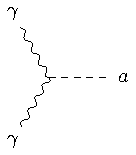
\includegraphics{diagrams/axion-biphoton.pdf}
		\caption{}
		\label{fig:axion-biphoton}
	\end{subfigure}
	\hspace{3em}
	\begin{subfigure}[]{0.2\textwidth}
		\centering
		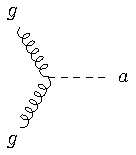
\includegraphics{diagrams/axion-bigluon.pdf}
		\caption{}
		\label{fig:axion-bigluon}
	\end{subfigure}
	\caption{Axion--photon and axion-gluon interaction vertices.}
	\label{fig:axion-vertices}
\end{figure}

The precise axion--matter interactions entering through the term $\LL_q'$ are model dependent, but generally have coupling strengths inversely proportional to the axion scale, $f_a$ \cite{Duffy_2009}.
However, all Peccei--Quinn axions interact with the gauge field though the last term in the Lagrangian \eqref{eqn:axion-Lagrangian}.
The last term is proportional to $\angbr{\tsbm F\wedge\tsbm F} = \ts F\wedge\ts F + \angbr{\tsbm G\wedge\tsbm G}$, where $\tsbm F = \ts F \oplus \tsbm G$ is the total gauge field split into the electromagnetic $\ts F$ and gluonic $\tsbm G$ sectors.
In perturbation theory, this corresponds to a Feynman vertex in which an axion and two photons $aγγ$, or an axion and two gluons $agg$ meet, as in figure~\ref{fig:axion-biphoton}.

The $aγγ$ interaction is strong where $\ts F\wedge\ts F = (\vec E \cdot \vec B)\,\vol$ is large.
This implies that axions may be generated from photons and vice-versa in the presence of strong electromagnetic fields.
Near a charged particle such as an electron, where the field is concentrated in a Coulomb potential, the $γ \leftrightarrow a$ conversion is best viewed as a scattering process, $γ + e^\pm \to e^\pm + a$, and is named the \emph{Primakoff effect} \cite[§\,93.1.3]{ParticleDataGroup-review-2020}.
The $agg$ vertex gives rise to interactions between axions and strongly-interacting hadronic matter (particularly pions and kaons) \cite{Cadamuro_2011}.
These interactions are universal to all axion models.
For \emph{leptonic} axion models with an electron interaction term $\LL_q$, there is also an axion--electron vertex.
This enables a Compton scattering process in addition to Primakoff scattering, both of which are shown in figure~\ref{fig:scattering-processes}.

\begin{figure}[h]
	\centering
	\begin{subfigure}[]{0.4\textwidth}
		\centering
		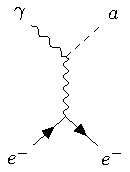
\includegraphics{diagrams/primakoff-process.pdf}
		\caption{Primakoff}
		\label{fig:Primakoff-scattering}
	\end{subfigure}
	\begin{subfigure}[]{0.4\textwidth}
		\centering
		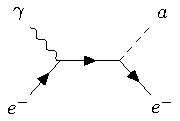
\includegraphics{diagrams/compton-process.pdf}
		\caption{Compton}
		\label{fig:Compton-scattering}
	\end{subfigure}
	\caption{Dominant axion processes with electrons (or positrons with arrows reversed) \cite{Cadamuro_2011}.
	Compton scattering only occurs for leptonic axions.}
	\label{fig:scattering-processes}
\end{figure}




\subsection{The Original Peccei--Quinn--Weinberg--Wilczek Axion}


The first proposed axion model, the Peccei--Quinn--Weinberg--Wilczek (PQWW) axion, \cite{Marsh_2016} implements the $\UPQ$ symmetry by supposing that the standard model possesses two Higgs fields $H_1$ and $H_2$ which couple differently to up and down quarks, instead of just one which couples to all quarks.
\note{Additionally, a complex scalar field $Φ$ is introduced as in the toy model, which is spontaneously broken and contains the axion as its angular degree of freedom.}
\note{
	WRONG: Apparently the complex scalar field is also a Higgs doublet!? [Marsh - Axion Cosmology, pg 7]
}
Denoting by $\bm ψ_\pm = \bm ψ_\pm^{(u)} \oplus \bm ψ_\pm^{(d)}$ the left- and right-handed quarks arranged into up-type and down-type parts, the two Higgs fields
\begin{align}
	\LL_\text{Yukawa} = \Re\qty(H_1 \bar{\bm ψ}_+ \mat m_u \bm ψ_-^{(u)} + H_2 \bar{\bm ψ}_+ \mat m_d \bm ψ_-^{(d)})
,\end{align}
where $\mat m_u$ and $\mat m_d$ are (non-square) matrices of Yukawa coupling constants.
The first Higgs field $H_1$ gives mass to the up-type quarks, and $H_2$ to down-type quarks.
The presence of the two Higgs fields lets $\LL_\text{Yukawa}$ be invariant under two independent chiral rotations of the up and down quarks, hence accomplishing the additional $\UPQ$ symmetry.

In this model, the axion scale $f_a$ is necessarily on the order of the electroweak scale, $f_\text{EW} \approx \SI{246}{\giga\eV}$ (which is the vacuum expectation value of the Higgs field).
The resulting axions are too massive ($m_a \approx \SI{25}{\kilo\eV}$) and too strongly interacting to agree with experiment.
In particular, the PQWW axion is ruled out by the non-observation of the kaon decay $K^+ \to π^+ + a$ in electron beam-dump experiments\footnotemark\ \cite{Peccei_1996,riordan1987search}.
\footnotetext{
	Beam-dump experiments involve firing high-energy protons into a high-absorption material in order to isolate neutral particles which are created from the decelerating protons and which propagate through the absorber.	
}
Any successful axion model must have a higher energy scale $f_a$ (i.e., lighter mass $m_a$) to be compatible with the constraints which excluded the PQWW model \cite{Marsh_2016}.


\subsection{Light Invisible Axion Models}

Axions with a larger energy scale $f_a \gg f_\text{EW}$ are light ($m_a \sim 1/f_a$), long lived (e.g., the rate of $a \to 2γ$ goes as $(f_a)^5$) and weakly interacting (couplings generally are suppressed by $1/f_a$).
In particular, their electromagnetic interactions are weak, rendering them invisible \cite{Peccei_1996,Marsh_2016}.
Such axion models generally fall into two classes:
\begin{itemize}
	\item \textit{The Kim--Shifman--Vainshtein--Zakharov (KSVZ) Axion} \\
	The KSVZ model introduces an additional massive quark $\bm q$ as well as the parent field $Φ$.
	\item \textit{The Dine--Fischler--Srednicki--Zhitnitsky (DFSZ) Axion} \\
	The DFSZ model contains two Higgs doubles like the PQWW model, but also contains a separate scalar parent field $Φ$.
	The DFSZ model contains the additional mass term
	\begin{align}
		\Re\qty(H_2\bar{\bm φ}_+\mat m_e\bm φ_-^{(e)})
	,\end{align}
	which is a Yukawa coupling between one of the Higgs doublets $H_2$, the left-handed leptons $\bm φ_+$, and the right-handed electron $\bm φ_-^{(e)}$, where $\mat m_e$ is the (non-square) matrix of Yukawa couplings.
	The $(H_2, \bm φ_-^{(e)})$ coupling gives rise to an axion--electron vertex, and hence DFSZ axions are leptonic and undergo Compton scattering (figure~\ref{fig:Compton-scattering}).

\end{itemize}


\section{Laboratory Bounds on Axions}

Axions have never been observed \cite[§\,91]{ParticleDataGroup-review-2020}.
The dynamics of the axion can be essentially parametrised by the mass $m_a$ and coupling $g_{aγγ}$ (and also the axion--electron coupling $g_{aee}$ for leptonic axions).
Negative axion detection experiments therefore serve to exclude specific regions of $(m_a, g_{aγγ})$ parameter space.
An exclusion plot of constraints from major laboratory experiments is shown in figure~\ref{fig:lab-bounds}.

\begin{figure}
	\centering
	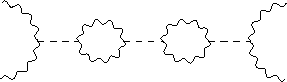
\includegraphics{diagrams/axion-photon-oscillation.pdf}
	\caption{Example axion--photon oscillation diagram.}
	\label{fig:axion-photon-oscillation}
\end{figure}


\subsubsection{Direct Axion Production}
In the presence of a strong, uniform electromagnetic field with $\vec E \parallel \vec B$ so that $\ts F\wedge\ts F$ is large, the $aγγ$ interaction is best viewed as an axion--photon oscillation, analogous to neutrino flavour oscillation (see figure~\ref{fig:axion-photon-oscillation}) \cite[§\,91.3.1]{ParticleDataGroup-review-2020}.
This suggests a scheme for detecting axions by `shining light through walls,' whereby a laser is beamed at an optical barrier in a strong magnetic field, and any generated axions (freely passing through the barrier) which oscillate back into photons on the other side are detected.
The first such experiment was performed in 1992 with a \SI{3.7}{\tesla} superconducting magnet over a length of \SI{4.4}{\meter}, and found that $|g_{aγγ}| < \SI{6.7e-7}{\per\giga\eV}$ for axions lighter than \SI{1}{\milli\eV} \cite{first-LSW-experiment}.
The current best limit from light-shining-though-walls (LSW) experiments, $|g_{aγγ}| < \SI{3.5e-8}{\per\giga\eV}$, was obtained in 2015 with two \SI{9}{\tesla} Large Hadron Collider dipole magnets \cite{best-LSW-experiment}, but there have been no positive axion detections.

Another consequence of axion--photon oscillation is that light suffers from dichroism\footnotemark\ and birefringence in a strong, uniform magnetic field $\vec B$.
The dichroism arises since the polarisation of light parallel to the magnetic field, $\vec E_\parallel$, where $\vec E \cdot \vec B$ is large, undergoes $aγγ$ oscillation and is depleted while $\vec E_\perp$ remains unaffected \cite[§\,91.3.2]{ParticleDataGroup-review-2020}.
A similar process results in birefringence, where linearly polarised light becomes elliptically polarised, but the experimental limits from dichroism experiments are stronger: $|g_{aγγ}| < \SI{3.6e-7}{\per\giga\eV}$ for sub-\si{\milli\eV} axions \cite{axion_dichromism}.
In 2006, a collaboration reported a false positive in a vacuum dichroism experiment, detecting axions with $m_a \approx \SI{1.3}{\milli\eV}$ and $g_{aγγ} = \SI{3e-6}{\per\giga\eV}$, but the detection was attributed to instrumental artefacts two years later \cite{birefringence_false_positive_2008}.


\footnotetext{
	Generally, \emph{dichroism} is the dependence of a medium's optical absorption on the polarization of light.
	In this case, the medium is the vacuum in regions of large $\ts F\wedge\ts F$.
}




\subsubsection{Detection of Solar Axions}

We also expect low-mass, weakly interacting particles to be produced in the astrophysical plasmas found inside stars.
Efforts have therefore been made to detect axions of solar origin.
In a strong macroscopic $\vec B$ field, axions (or indeed, any axion-like particles with a two-photon vertex) may be converted into x-rays via a reverse Primakoff process, $a + e^\pm \to e^\pm + γ$.
With standard solar models, the expected axion flux on Earth is
\begin{align}
	φ_\odot \approx 3.8\times10^{11}\,(10^{10}\,\si{\giga\eV}\,|g_{aγγ}|)^2\,\si{\per\square\cm\per\s}
,\end{align}
which is significant and detectable for axions with $|g_{aγγ}| \gtrsim 10^{-11}\,\si{\per\giga\eV}$ \cite{solar-axion-flux_2007}.

The Tokyo axion helioscope, initially constructed in 1995 and then continuously upgraded, utilised a \SI{4}{\tesla} superconducting magnet on a sun-tracking mount to detect solar axions.
In 2008, it was reported that its negative results implied a limit $|g_{aγγ}| < \SI{6e-10}{\per\giga\eV}$ for sub-\si{\milli\eV} axions \cite{Tokyo-axion-helioscope_2008}.
More recently, the CERN Axion Solar Telescope used a decommissioned \SI{9}{\tesla} LHC dipole magnet in a similar helioscope apparatus to establish a stronger limit: $|g_{aγγ}| < \SI{6.6e-11}{\per\giga\eV}$, though only for axions of mass $m_a < \SI{0.03}{\eV}$ \cite{CAST-helioscope_2017}.


\begin{figure}
	\centering
	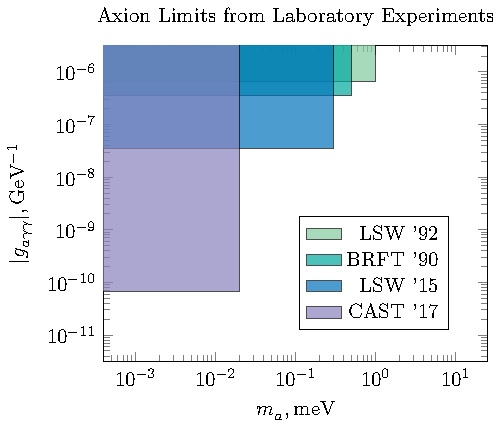
\includegraphics{diagrams/lab-bounds.pdf}
	\caption{Limits on axion mass $m_a$ and photon coupling {}$g_{aγγ}$ from laboratory experiments. Shaded regions are experimentally excluded.
		(LSW '92 \cite{first-LSW-experiment},
		BRFT '90 \cite{axion_dichromism},
		LSW '15 \cite{best-LSW-experiment},
		CAST '17 \cite{CAST-helioscope_2017})
	}
	\label{fig:lab-bounds}
\end{figure}

Further laboratory experiments to detect axions are under way (e.g., \cite{further-lab-experiments_2017}, \cite[§\,5.3]{Irastorza_2018}), but direct detection on Earth is not the only experimental probe available.
Axions may have significant roles in stellar evolution, the universe's early history and as dark matter, placing them in the domain of cosmology.